\chapter{Dados e gráficos}
\markboth{Módulo 8}{}

\section*{Habilidades do SAEB}

\begin{itemize}
\item Ler/identificar ou comparar dados estatísticos expressos em tabelas
(simples ou de dupla entrada).

\item Ler/identificar ou comparar dados estatísticos expressos em gráficos
(barras simples ou agrupadas, colunas simples ou agrupadas, pictóricos
ou de linhas).

\item Resolver problemas que envolvam dados apresentados, tabelas (simples ou
de dupla entrada) ou gráficos estatísticos (barras simples ou agrupadas,
colunas simples ou agrupadas, pictóricos ou de linhas).
\end{itemize}

\subsection{Habilidade da BNCC}

\begin{itemize}
  \item 
 EF03MA27.
\end{itemize}

\pagebreak

\conteudo{
\begin{itemize}
\item
\textsc{Gráfico de colunas ou barras}
\end{itemize}

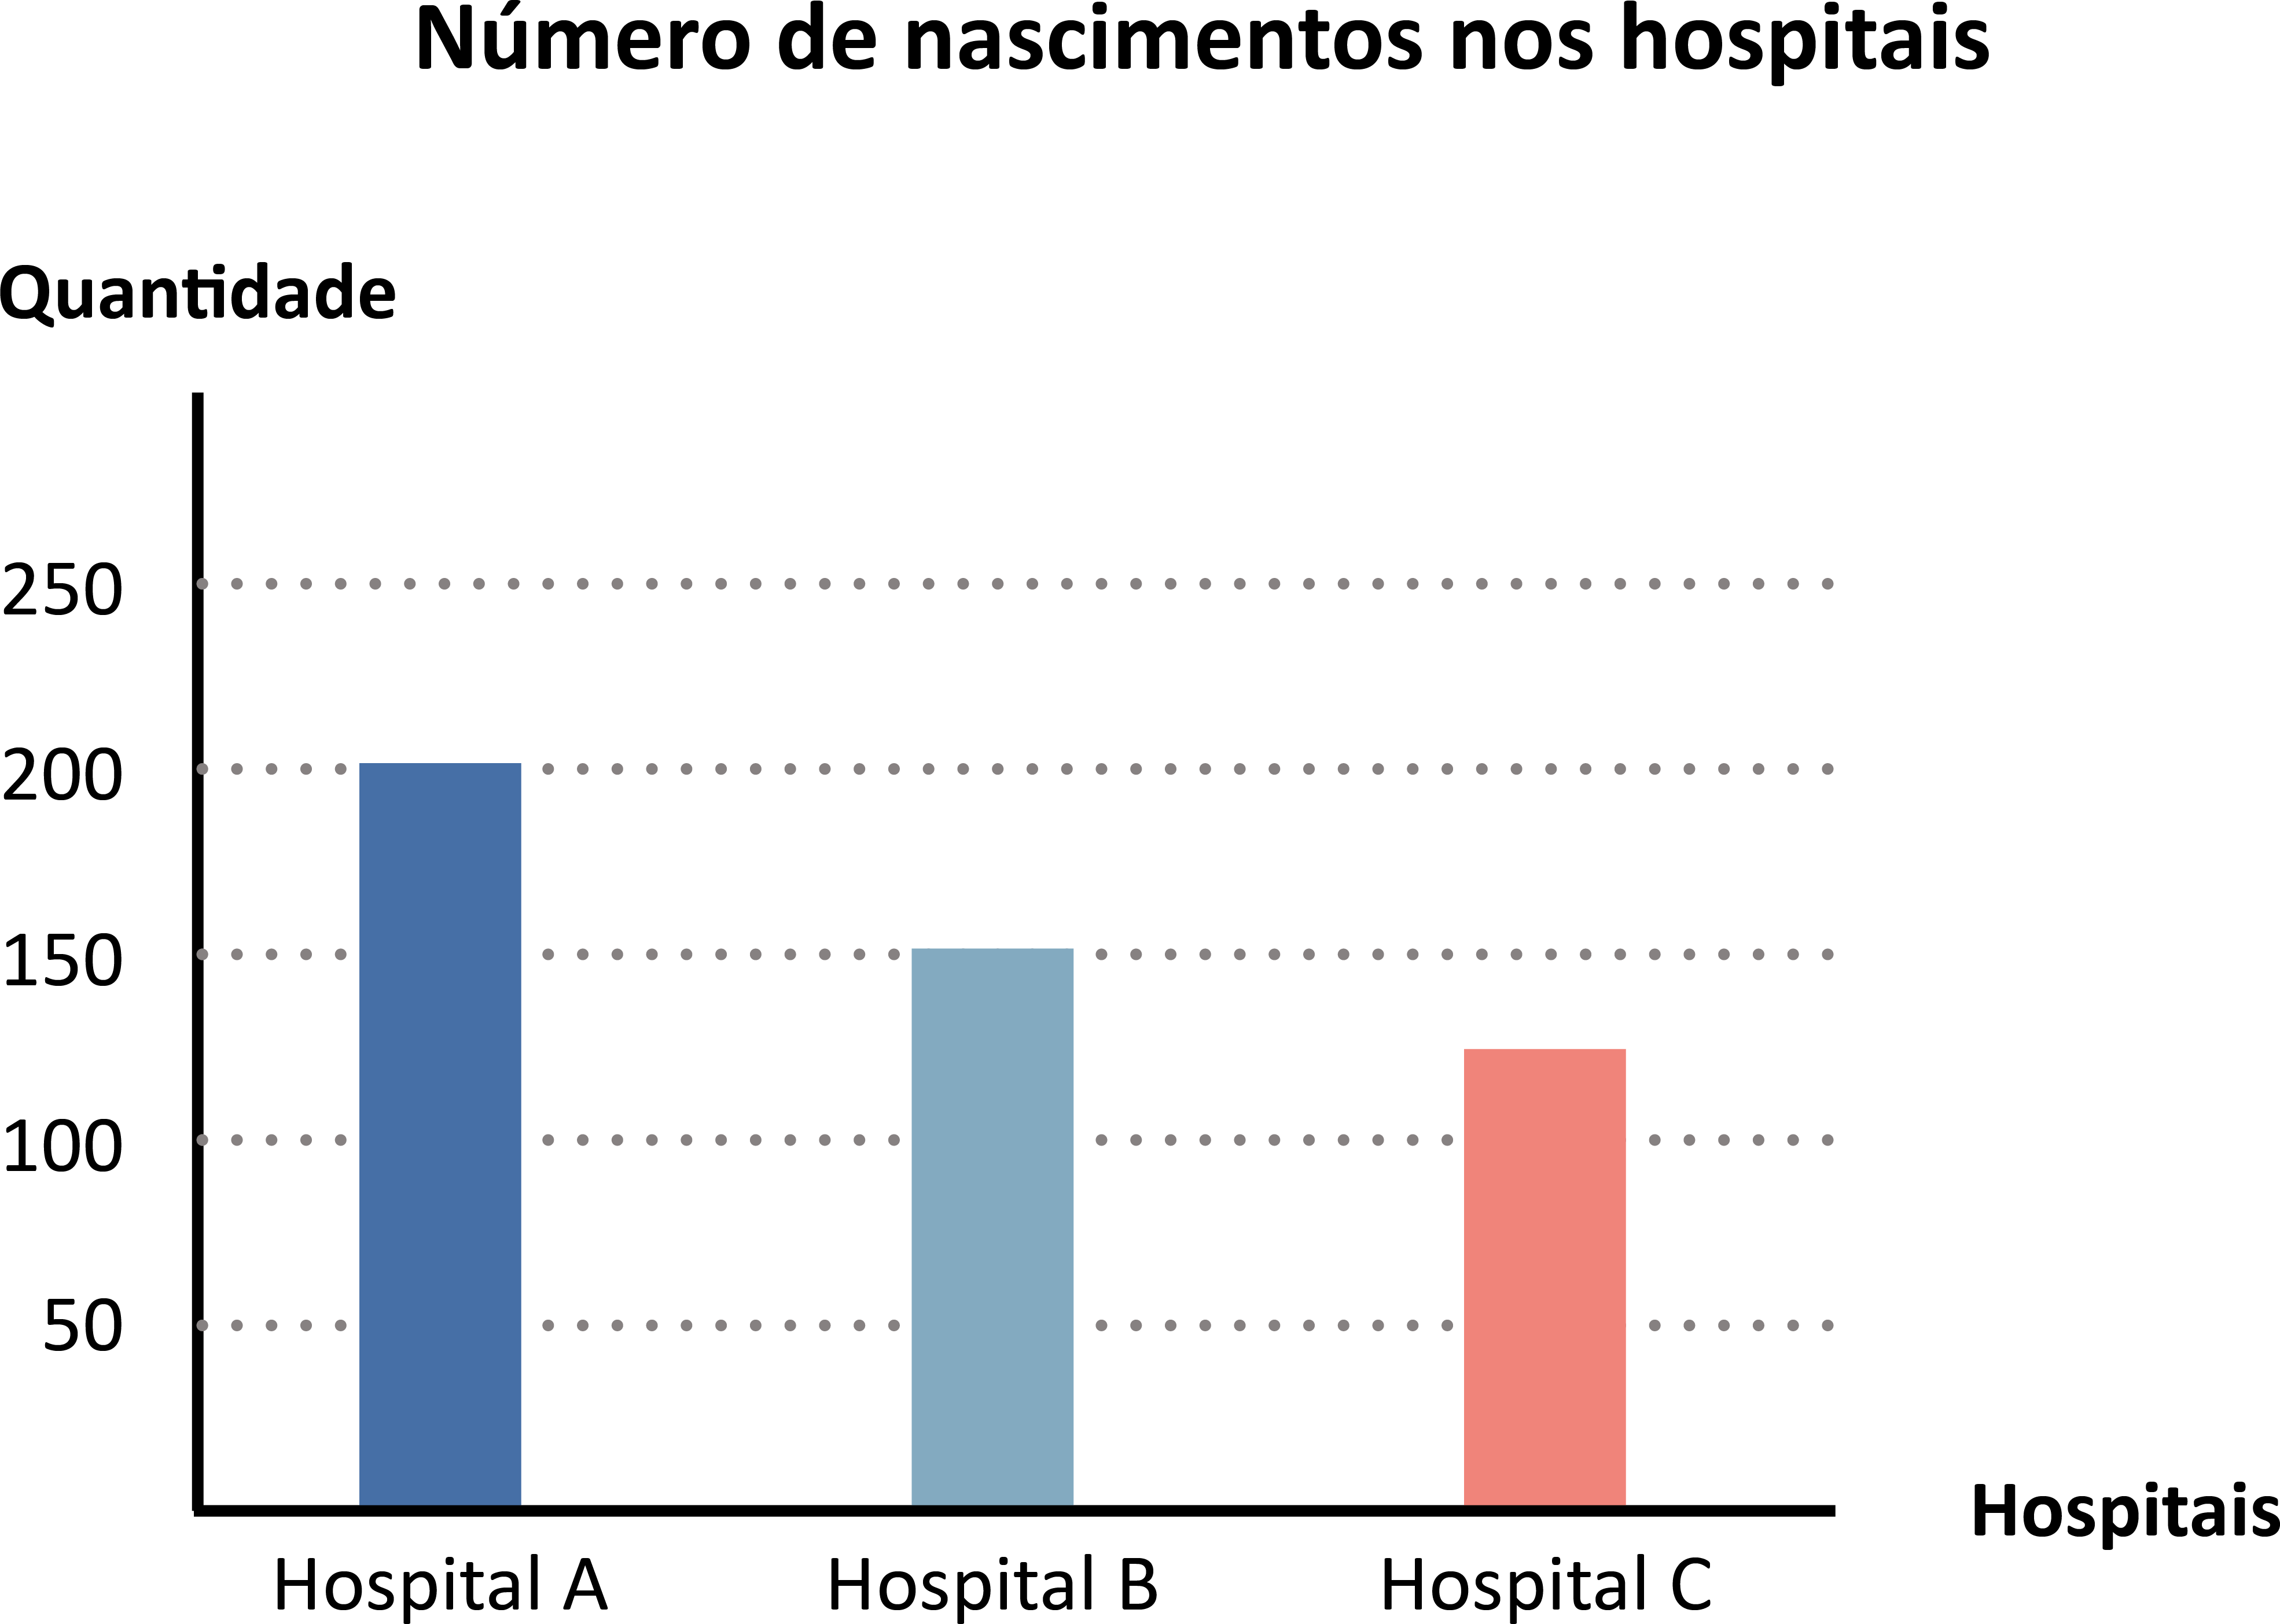
\includegraphics[width=0.9\textwidth]{./media/image75.png}


\begin{itemize}
\item
\textsc{Pictograma}
\end{itemize}

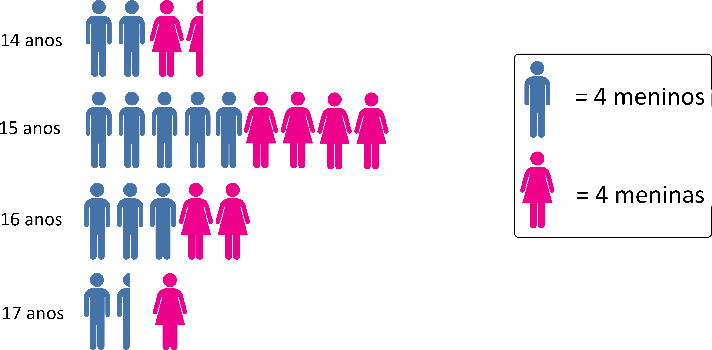
\includegraphics[width=\textwidth]{./media/image76.png}
}

\pagebreak

\conteudo{
\begin{itemize}
\item
\textsc{Gráfico de linhas}
\end{itemize}

\vspace{2em}
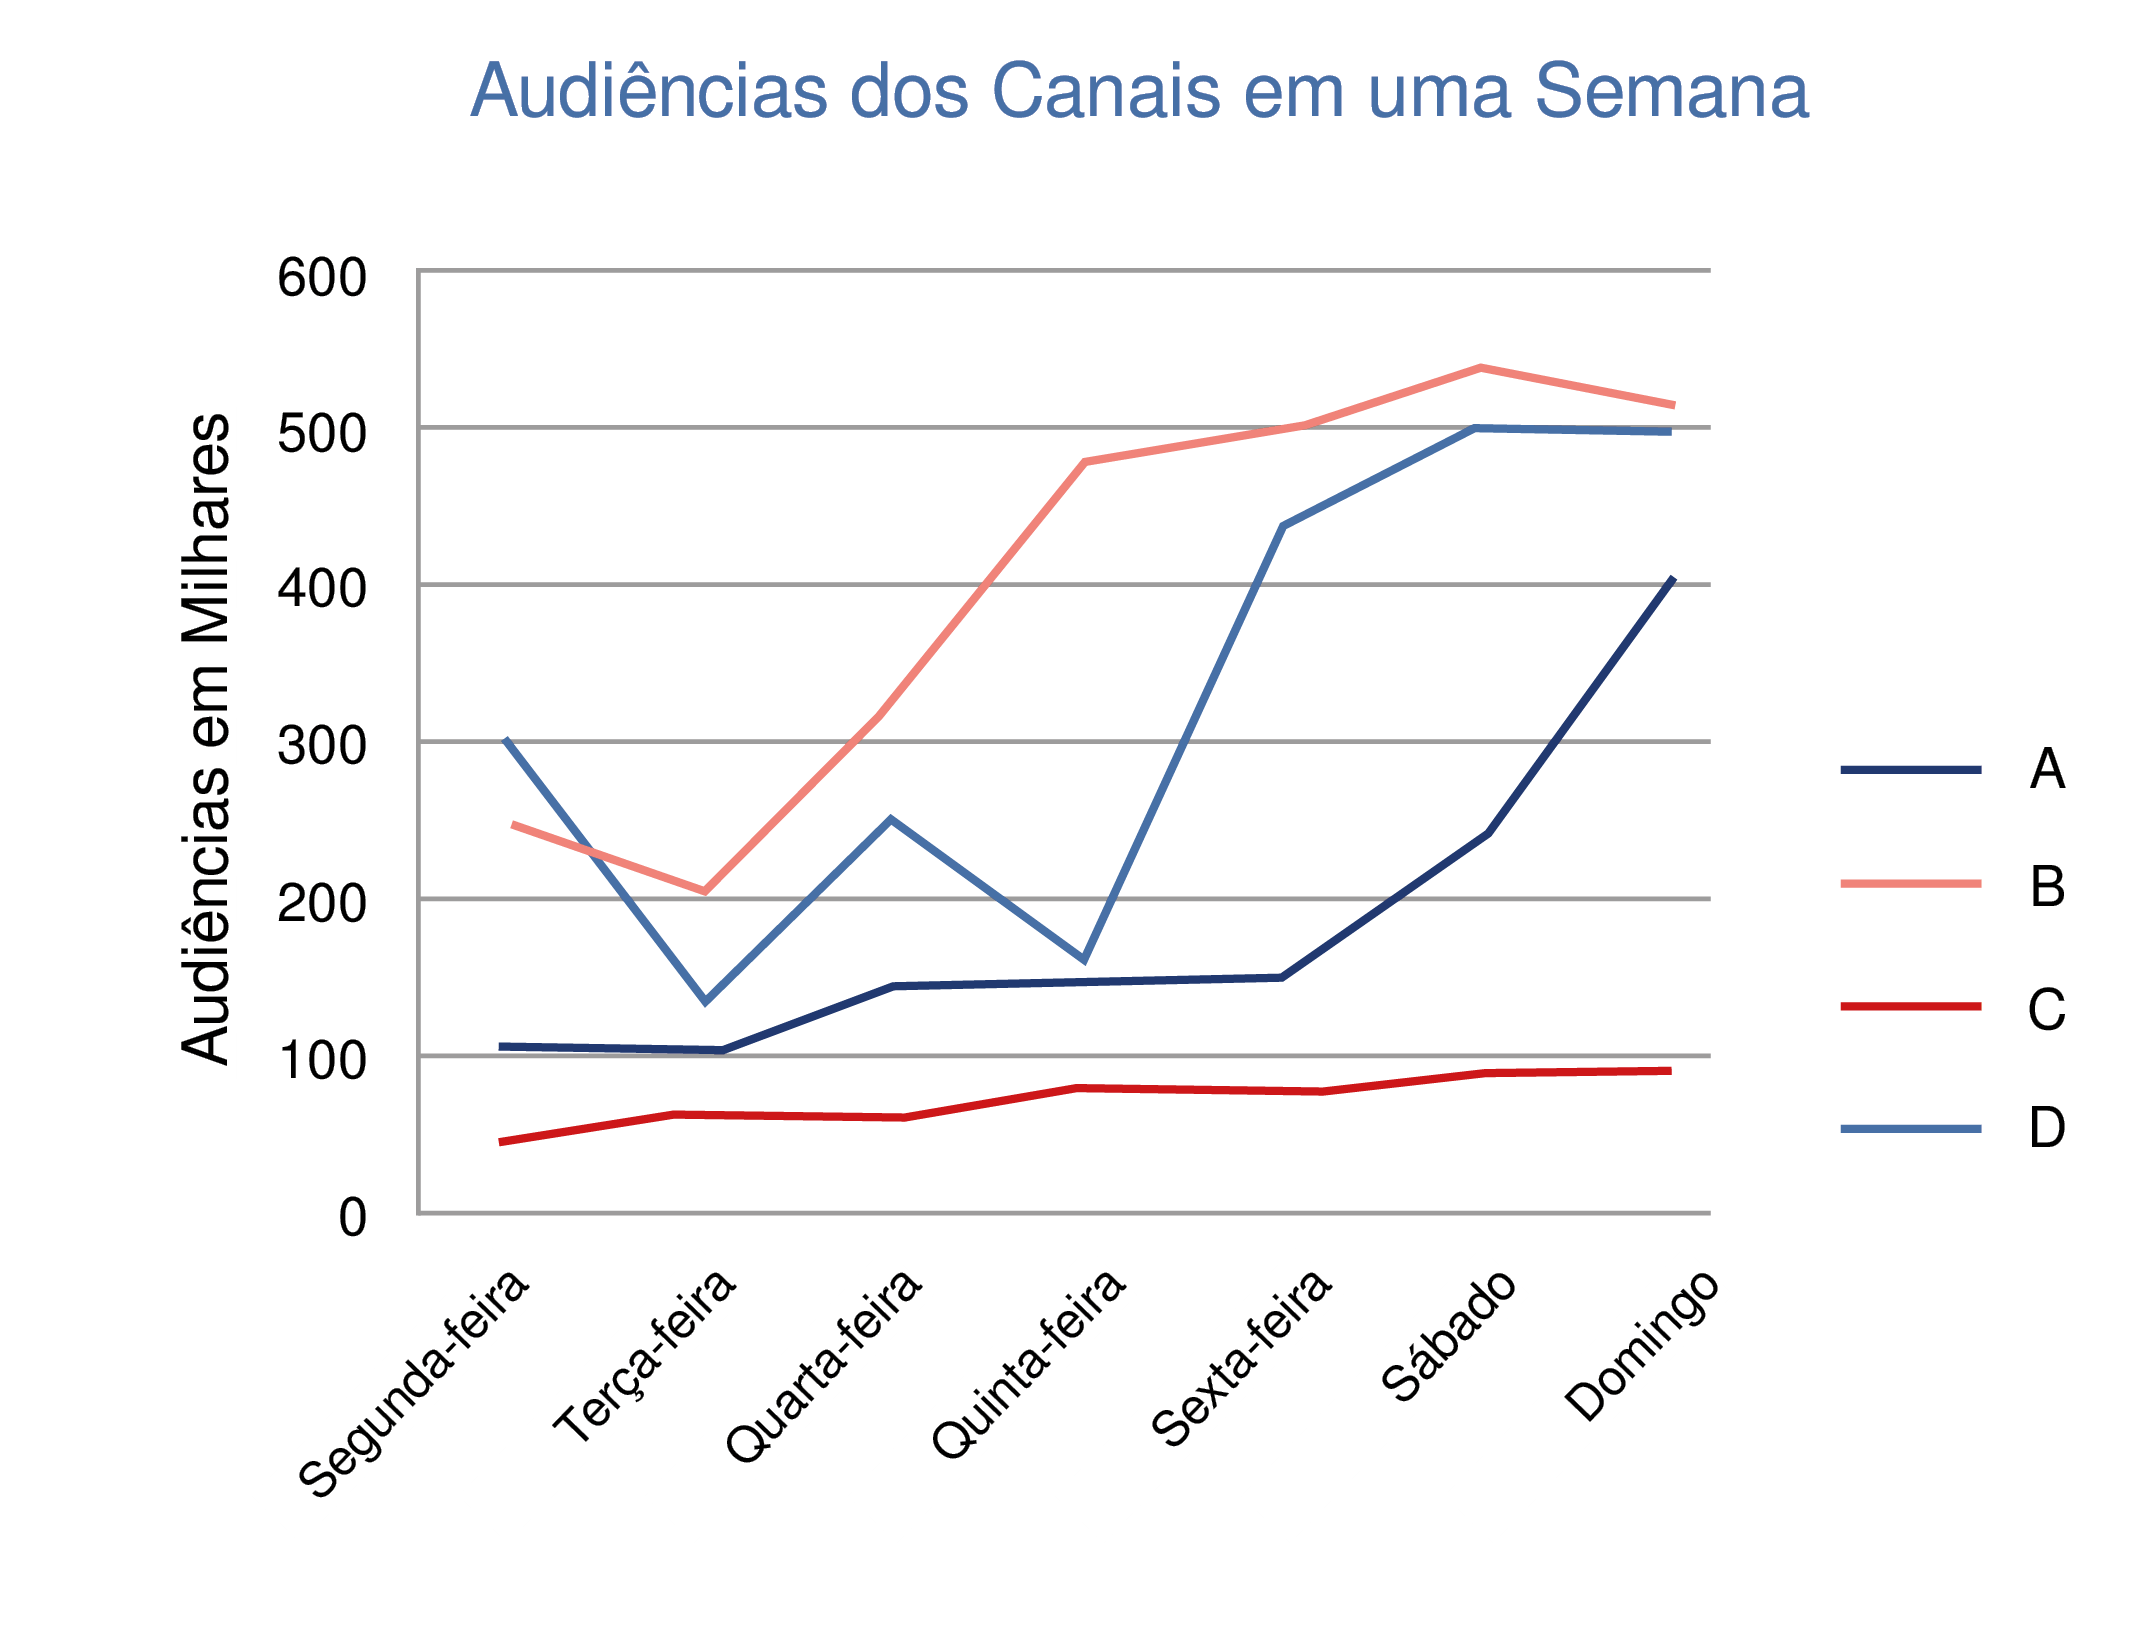
\includegraphics[width=0.8\textwidth]{./media/image77.png}

\begin{itemize}
\item
  \textsc{Gráfico de setores}
\end{itemize}


\includegraphics[width=0.8\textwidth]{./media/image78.png}
}

\section*{Atividades}

\num{1} Após um longo período de férias, as aulas de Regina voltaram a acontecer.
No primeiro dia de aula, a professora fez uma pesquisa sobre as viagens de seus alunos durante o período de recesso. Cada aluno foi
orientado a escolher somente um lugar e, após escutar todas as respostas,
a professora montou o seguinte gráfico com os dados fornecidos pelos alunos:

\begin{figure}[htpb!]
\centering
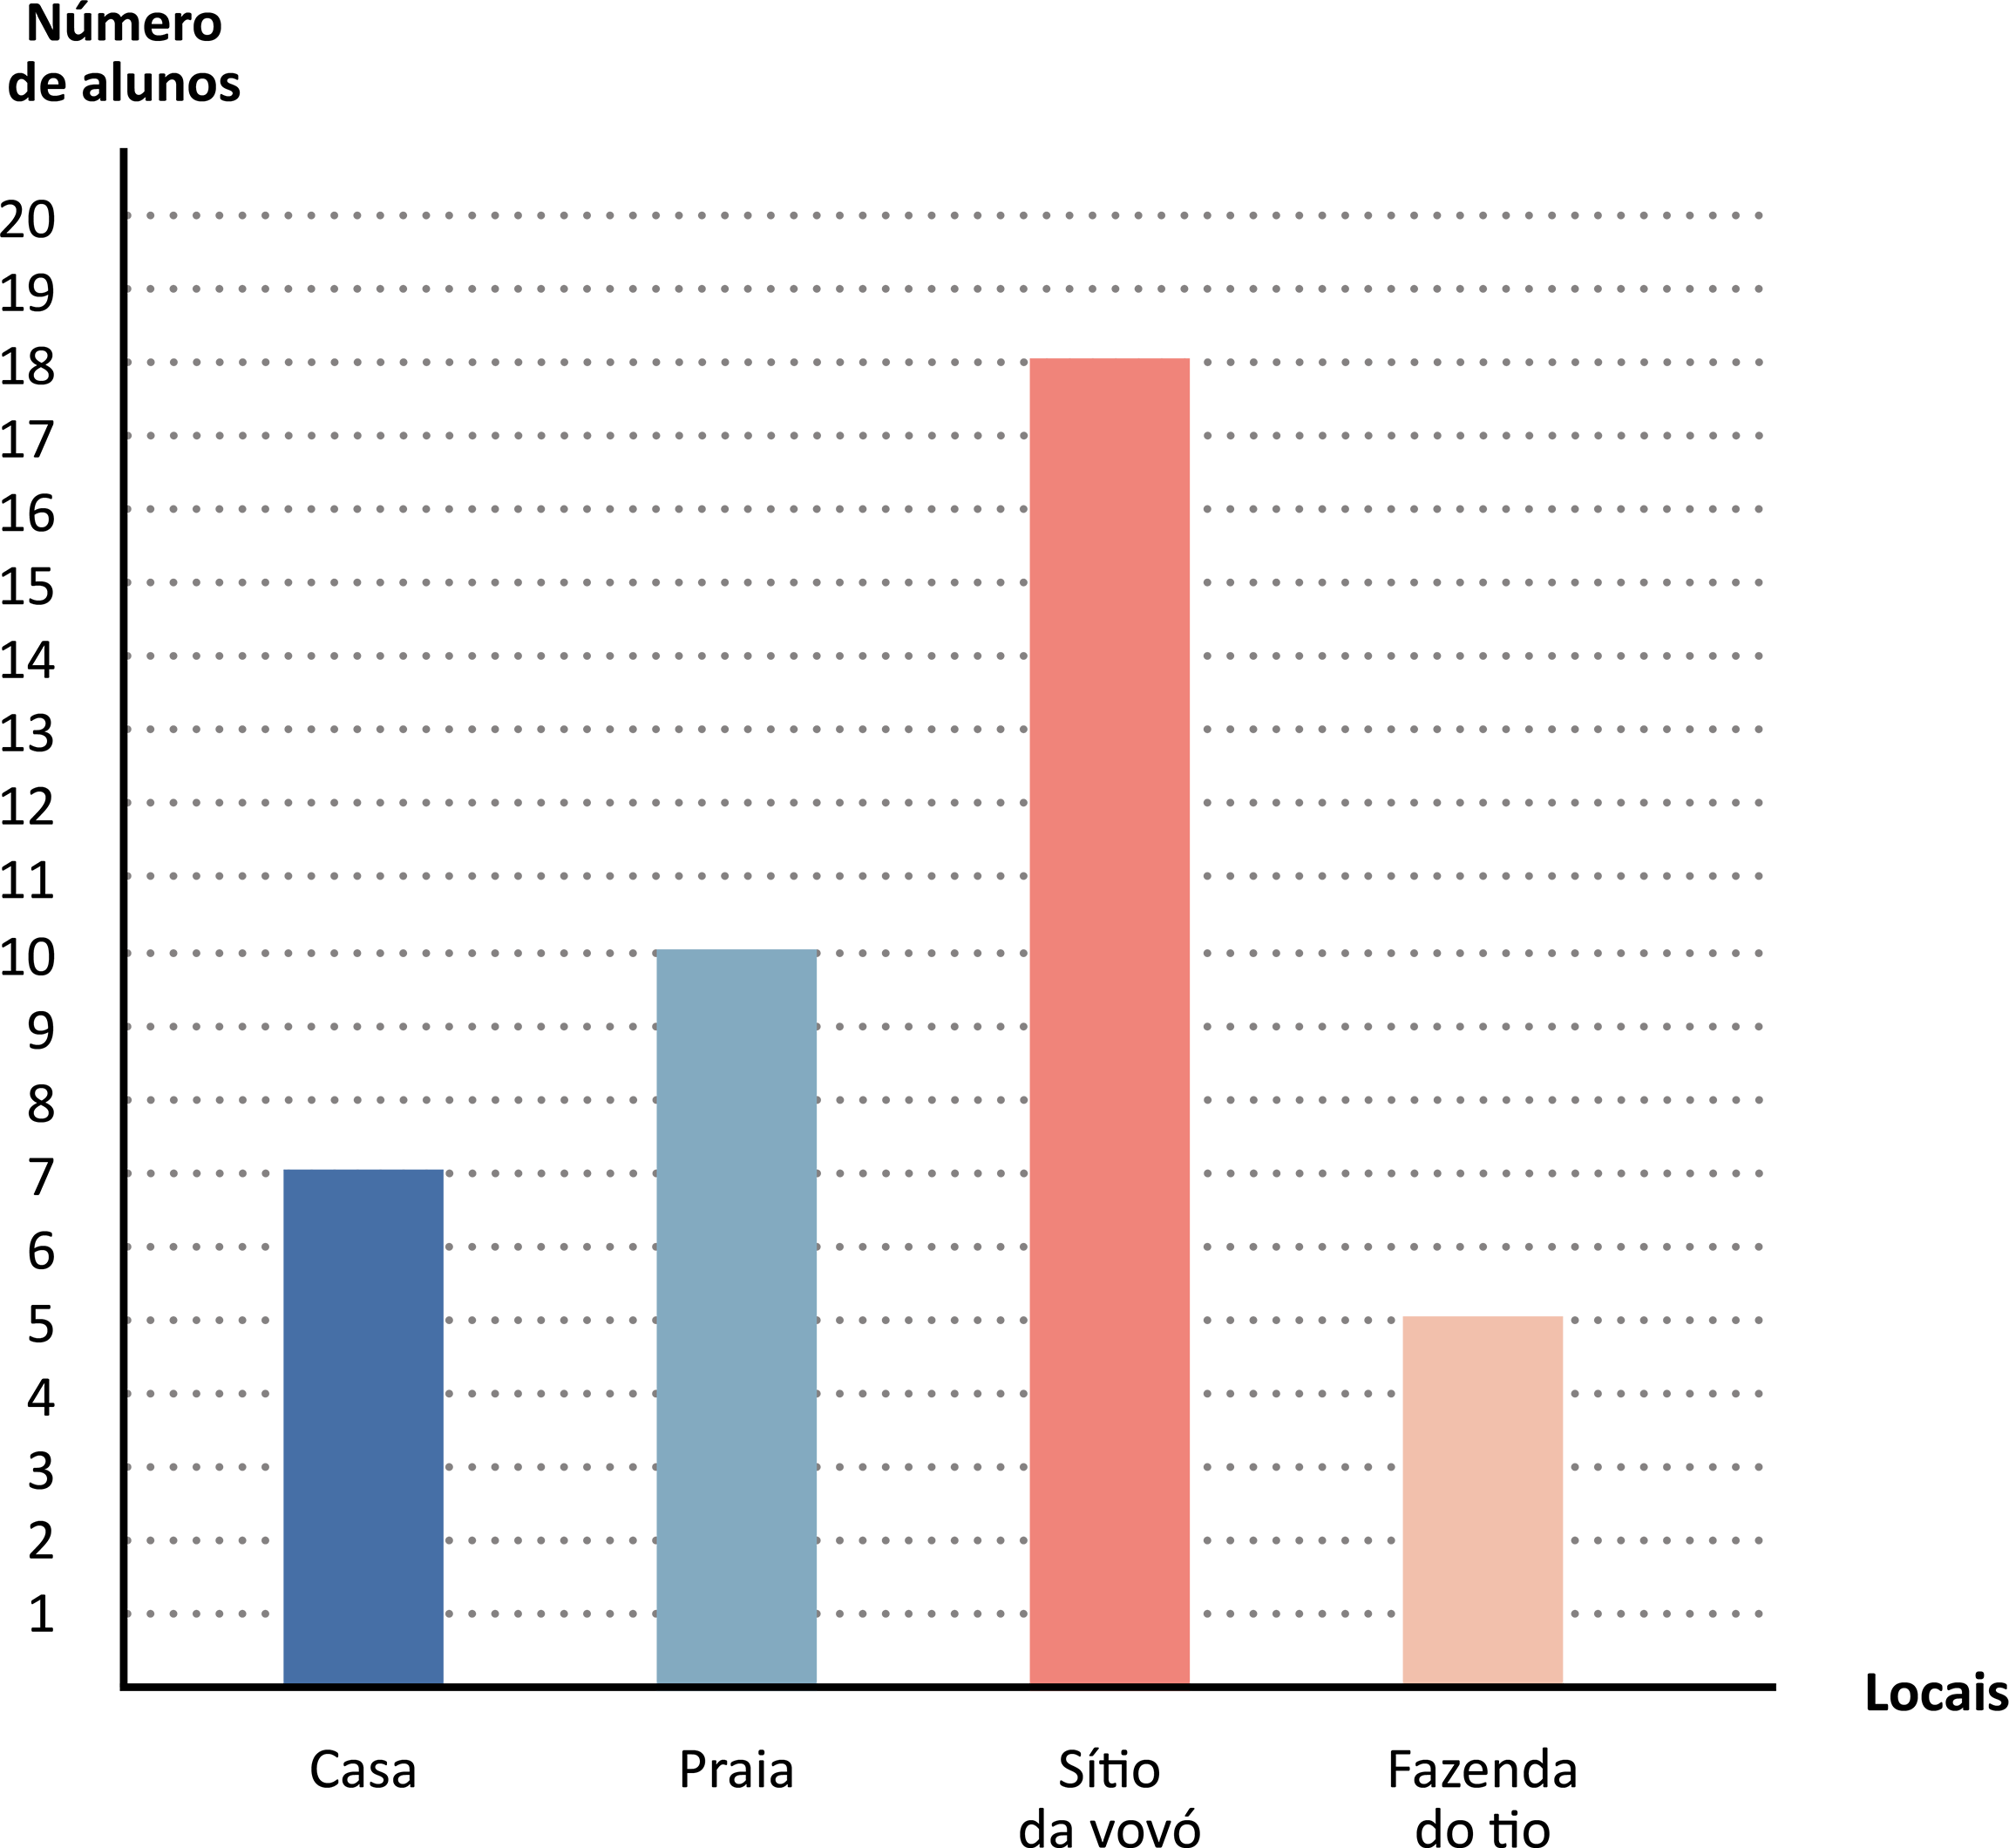
\includegraphics[width=\textwidth]{./media/image79.png}
\end{figure}

Qual foi a resposta menos dada pelos alunos segundo esse gráfico?
\reduline{Observando o gráfico, percebemos que a resposta que menos apareceu foi a
fazenda do tio, com 5 aparições.\hfill}

\num{2} Durante uma aula de matemática sobre estatística, os alunos fizeram uma
pesquisa entre eles para consolidar seus aprendizados. A turma fez uma
pergunta a todos os alunos sobre o tipo de filme preferido, e cada aluno
poderia dar apenas uma resposta. Após essa coleta de respostas, eles
fizeram a tabela mostrando as respostas dos meninos e das
meninas:

\begin{center}
\begin{tabular}{l|ll}
\hline
\multirow{2}{*}{\textbf{Tipo de filme}} & \multicolumn{2}{l}{\textbf{Número de votos}} \\ \cline{2-3} 
 & \multicolumn{1}{l|}{\textbf{Meninas}} & \textbf{Meninos} \\ \hline
\textbf{Aventura} & \multicolumn{1}{l|}{6} & 15 \\ \hline
\textbf{Comédia} & \multicolumn{1}{l|}{4} & 2 \\ \hline
\textbf{Desenho animado} & \multicolumn{1}{l|}{6} & 1 \\ \hline
\textbf{Terror} & \multicolumn{1}{l|}{2} & 4 \\ \hline
\end{tabular}
\end{center}

Observando o quadro, qual o tipo de filme de que meninas gostam menos? 
\reduline{As meninas gostam menos de filme de terror, com 1 voto apenas.\hfill}

\num{3} Após todas as rodadas de um campeonato de futebol, os organizadores
apresentaram um gráfico com o número de pontos que cada
time obteve.

\begin{figure}[htpb!]
\centering

\includegraphics[width=\textwidth]{./media/image80.png}
\end{figure}

Observando atentamente o gráfico, podemos concluir que o time D fez quantos pontos?
\reduline{Olhando atentamente para o gráfico, temos que o time D fez 50 pontos
durante esse campeonato.\hfill}

\num{4} Durante um evento de automobilismo, foram colhidas as informações sobre o número de carros
que entraram e também a quantidade de pessoas que estavam em cada carro.
Esses dados foram colocados em uma tabela.

\begin{longtable}[]{@{}ll@{}}
\toprule
\hline
\textbf{Número de pessoas por carro} & \textbf{Quantidade de carros}
\tabularnewline
\hline
\midrule
\endhead
\textbf{Apenas 1 pessoa} & 5\tabularnewline
\hline
\textbf{2 pessoas} & 12\tabularnewline
\hline
\textbf{3 pessoas} & 15\tabularnewline
\hline
\textbf{4 pessoas} & 7\tabularnewline
\hline
\textbf{5 pessoas} & 5\tabularnewline
\bottomrule
\end{longtable}

Construa um gráfico de colunas com os dados da tabela.

\begin{figure}[htpb!]
\centering
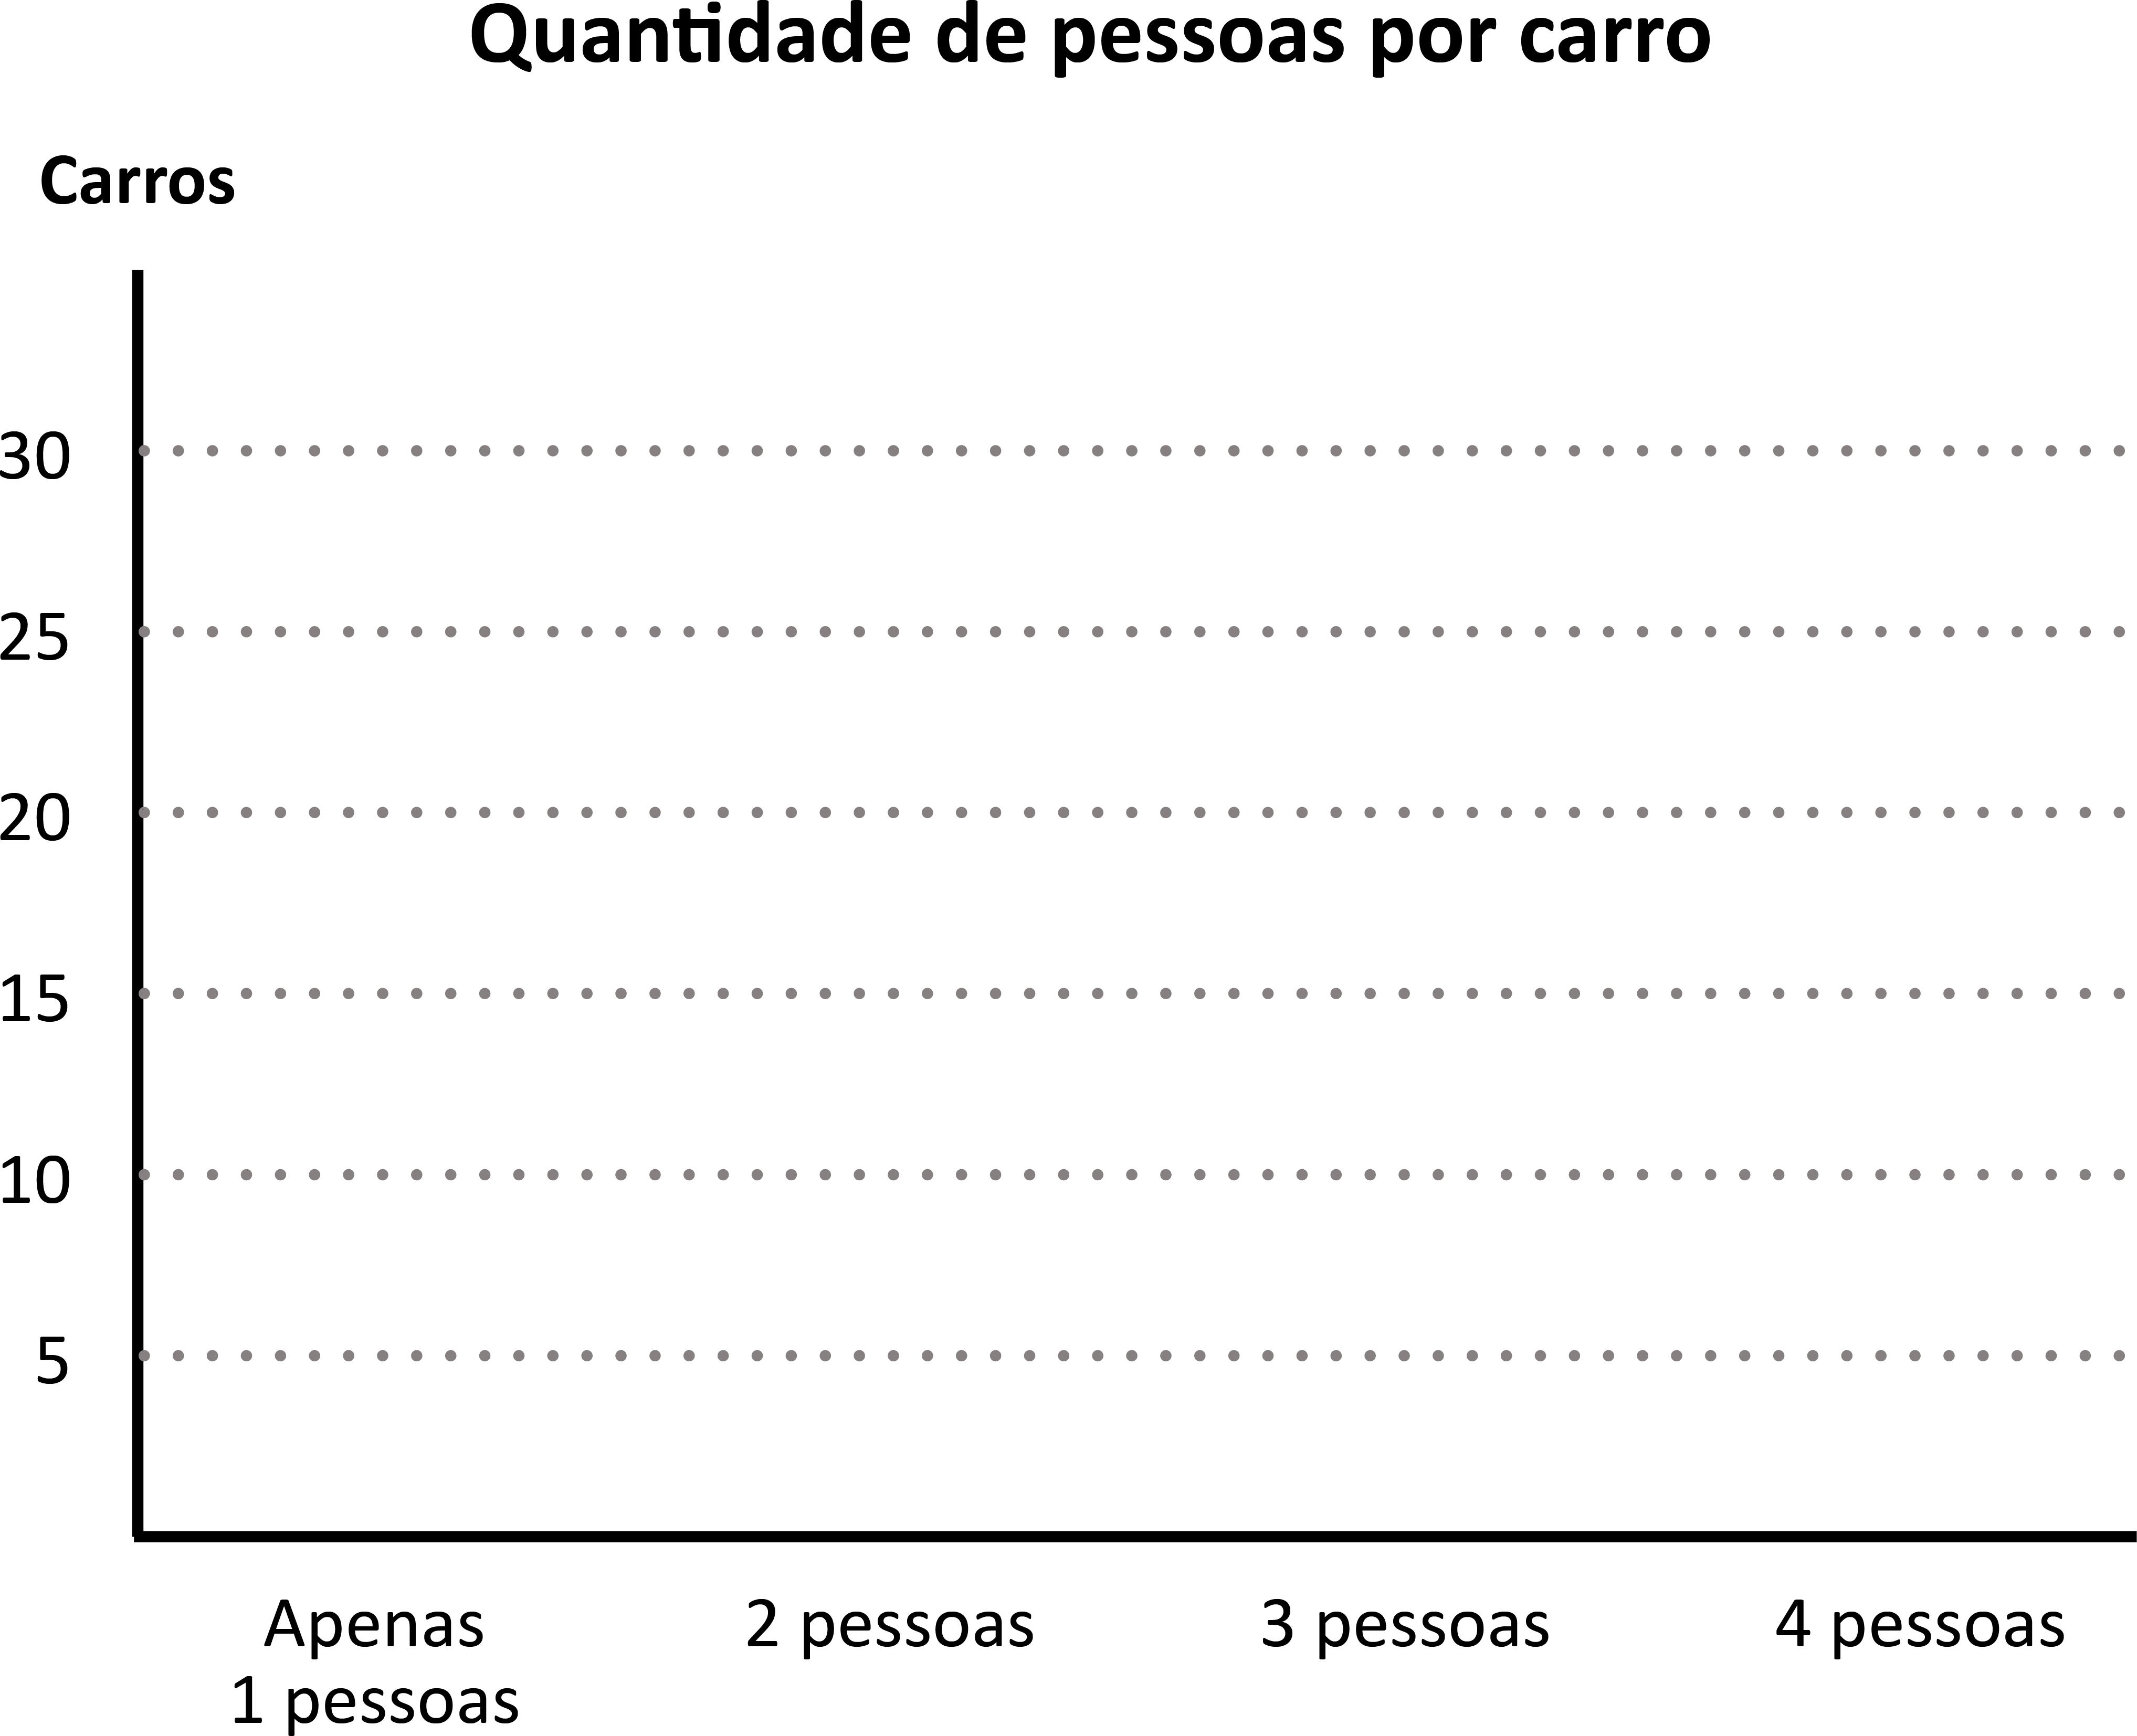
\includegraphics[width=\textwidth]{./media/image81.png}
\end{figure}
%NOTE. Atividade sem resposta.

\num{5} Uma empresa de telefonia fez uma pesquisa para saber qual é o índice de
satisfação de seus clientes em relação aos serviços prestados. Esses dados foram
colocados em uma tabela.

\begin{figure}[htpb!]
\centering

\includegraphics[width=.8\textwidth]{./media/image82.png}
\end{figure}

Pela análise do gráfico, qual foi o número de pessoas que
responderam Bom ou Normal? 
\reduline{120 + 150 = Total: 270.\hfill}

\num{6} O quadro mostra a quantidade de abacaxis vendidos por um feirante
durante alguns dias do mês de maio.

\begin{longtable}[]{@{}ll@{}}
\toprule
\hline
\textbf{Dia} & \textbf{Quantidade de abacaxis vendidos}\tabularnewline
\hline
\midrule
\endhead
04/05 & 89\tabularnewline
\hline
05/05 & 68\tabularnewline
\hline
06/05 & 52\tabularnewline
\hline
07/05 & 71\tabularnewline
\bottomrule
\end{longtable}

Analisando os dados, responda ao que se pede em cada item.

\pagebreak

\begin{escolha}
\item Quantos abacaxis foram vendidos nos dias 05/05 e 06/05?
\reduline{68 + 52 = 120.\hfill}

\item Em que dia a venda de abacaxis foi a maior?
\reduline{O dia com maior venda foi 04/05, com 89 abacaxis.\hfill}

\item Em que dia a venda de abacaxis foi a menor?
\reduline{O dia com menor venda foi 06/05, com 52 abacaxis.\hfill}
\end{escolha}

\num{7} Uma empresa de doces resolveu contratar um matemático que realizasse uma
pesquisa para verificar o tipo preferido de sobremesa das pessoas que
frequentavam determinado supermercado. Os entrevistados poderiam dar
apenas uma resposta dentre as oferecidas na pesquisa e, após contagem dos
votos sobre a preferência, o matemático apresentou o quadro a seguir
para a empresa que o contratou.

\begin{longtable}[]{@{}ll@{}}
\toprule
\hline
\textbf{Sobremesa} & \textbf{Total de votos}\tabularnewline
\hline
\midrule
\endhead
\textbf{Pudim} & 35\tabularnewline
\hline
\textbf{Sorvete} & 20\tabularnewline
\hline
\textbf{Doce de leite} & 22\tabularnewline
\hline
\textbf{Goiabada com queijo} & 10\tabularnewline
\hline
\textbf{Salada de frutas} & 13\tabularnewline
\hline
\bottomrule
\end{longtable}

Analisando o gráfico apresentado, responda:

\begin{escolha}
\item Qual a sobremesa menos votada?
\reduline{A sobremesa menos votada foi a goiabada com queijo.\hfill}

\item Qual a sobremesa mais votada?
\reduline{A sobremesa mais votada foi o pudim.\hfill}

\item Construa uma sequência crescente dos números apresentados na tabela.
\reduline{10;13;20;22;35.\hfill}

\item Após construir a sequência crescente, qual número ficou na posição central?
\reduline{O número que ocupa a posição central na sequência é o 20.\hfill}
\end{escolha}

\num{8} O professor de educação física apresentou os dados da quantidade de gols
marcados pelos 4 times que dispuraram o interclasses de futebol no ano
corrente.

\begin{figure}[htpb!]
\centering
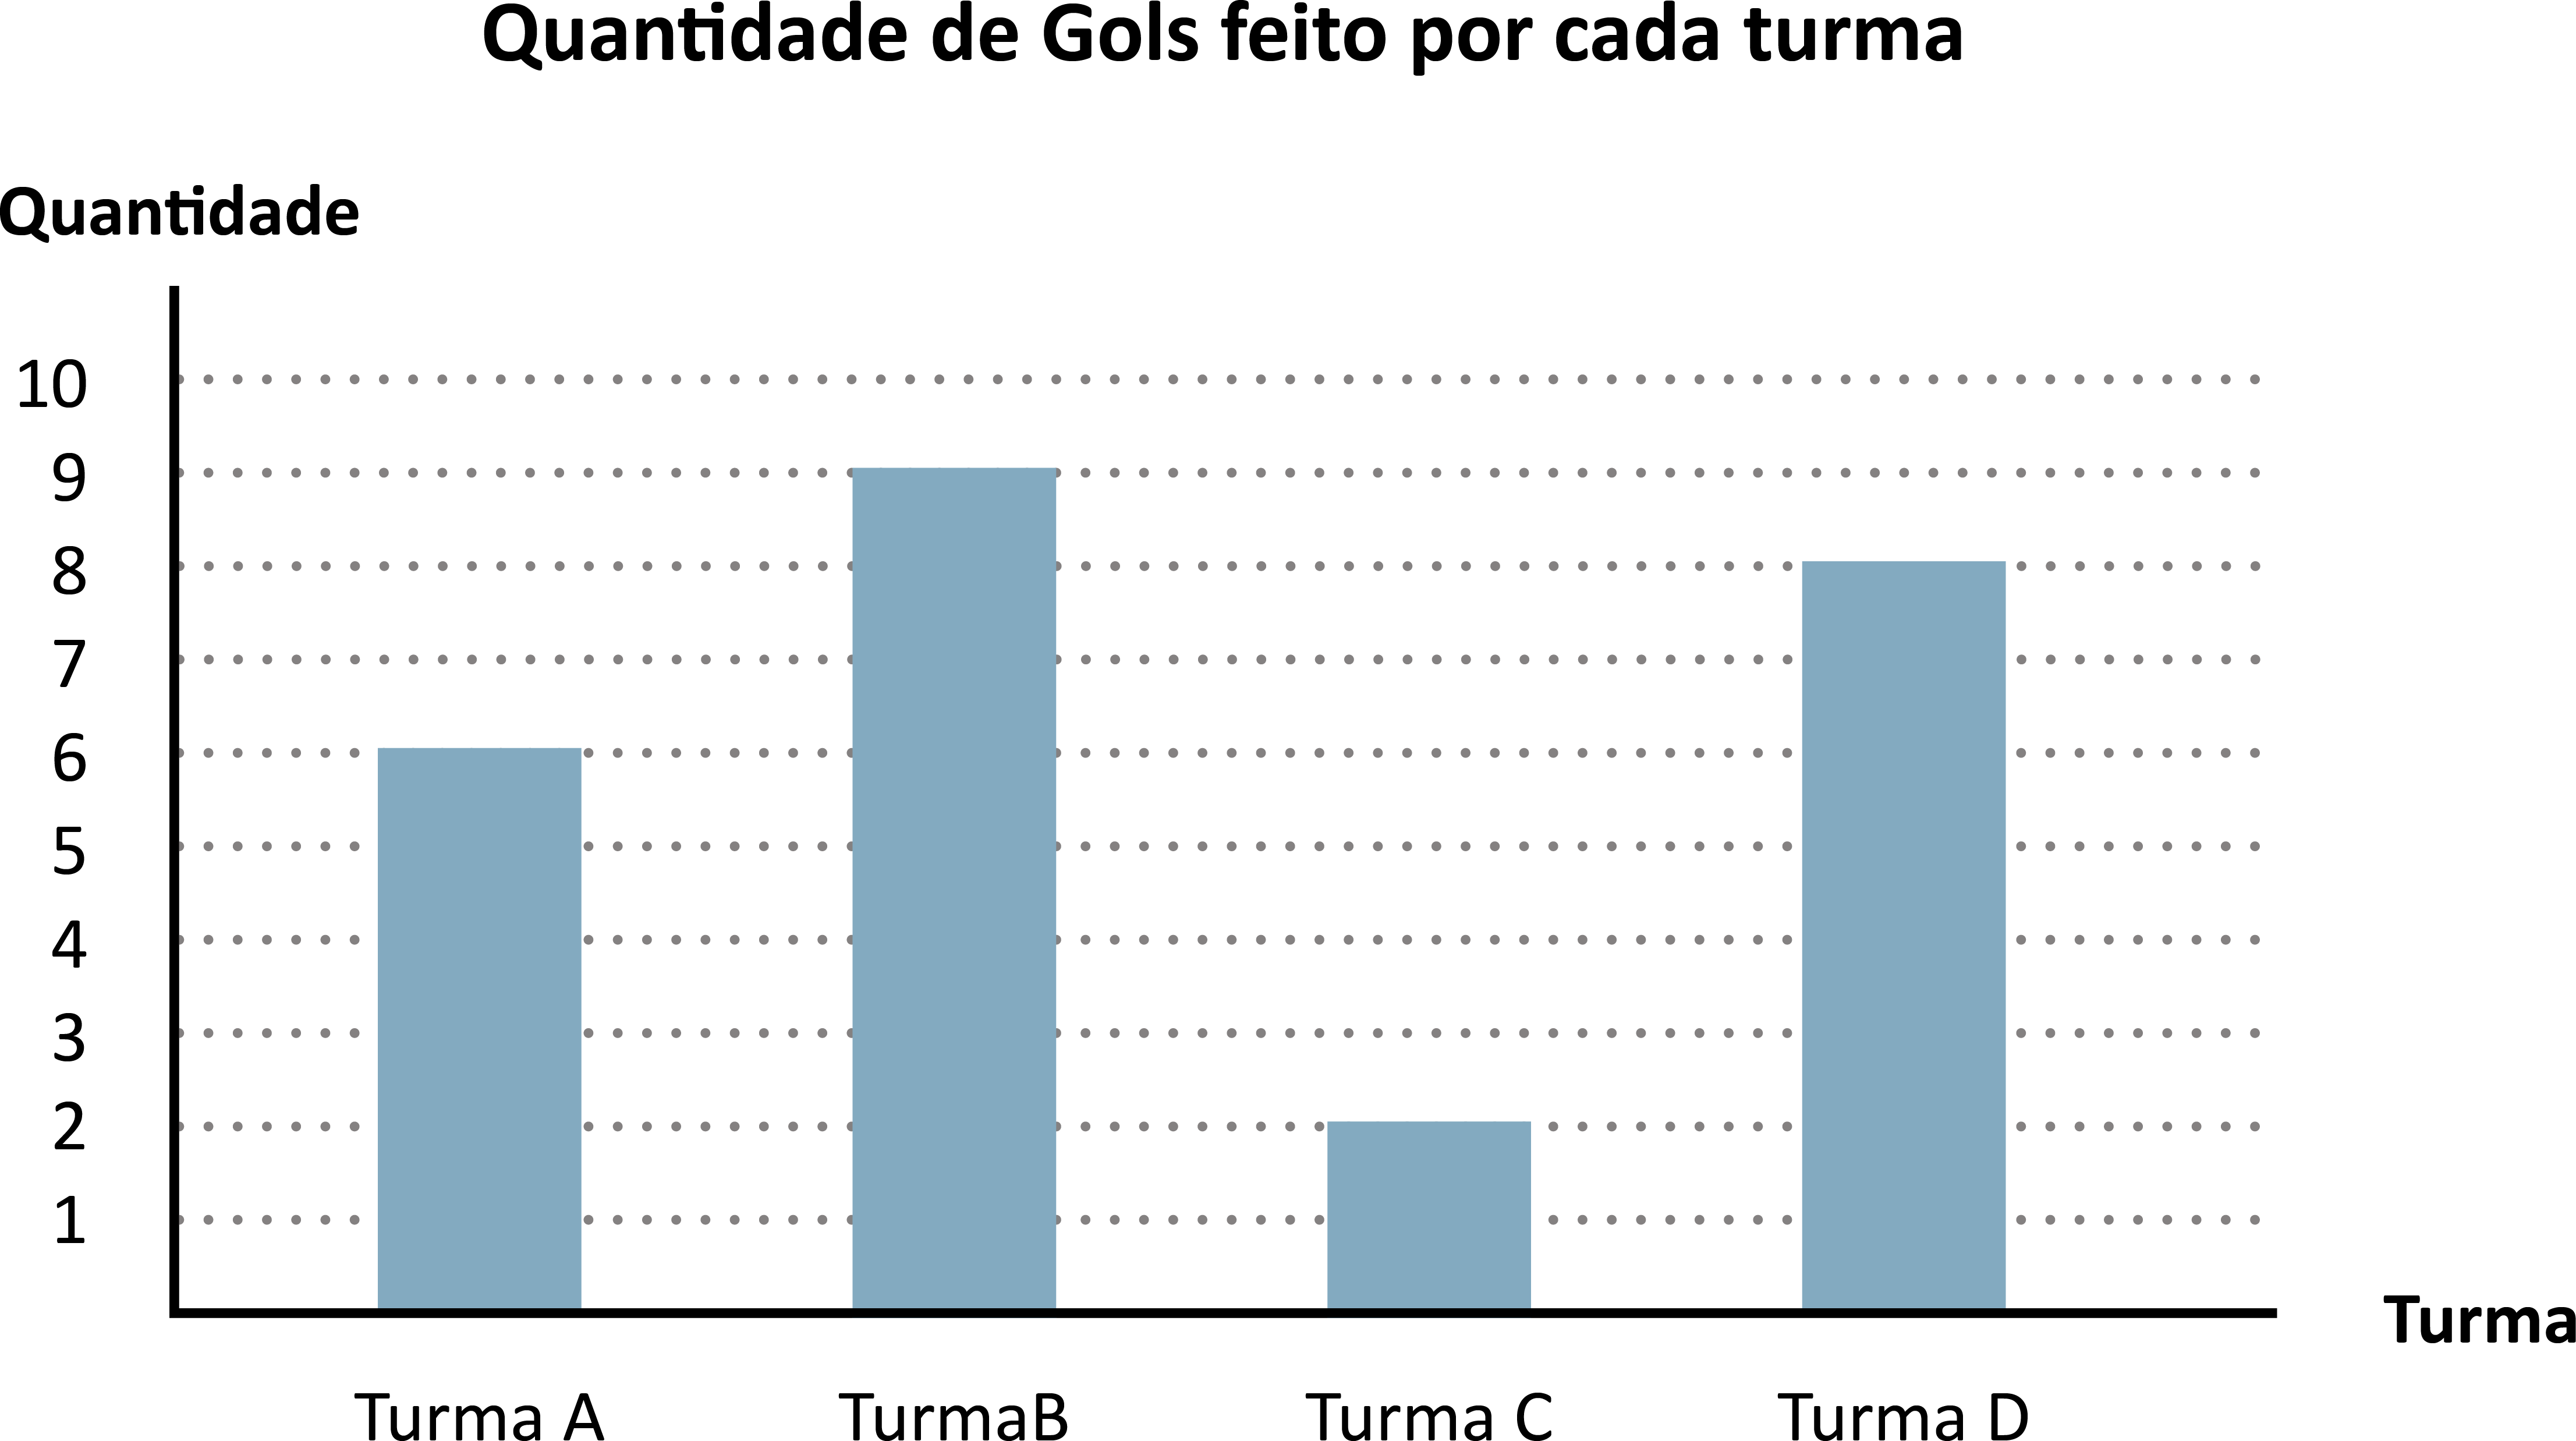
\includegraphics[width=.8\textwidth]{./media/image83.png}
\end{figure}

Analisando atentamente o gráfico, responda:

\begin{escolha}
\item Qual turma fez a maior quantidade de gols? E qual foi a quantidade que fizeram?
\reduline{A turma que fez a maior quantidade de gols foi a B, com 9 gols.\hfill}

\item Quais turmas fizeram um número de gols maior que 6?
\reduline{As turmas que fizeram um número de gols maior que 6 foram as turmas B
  e D. Reforce com os alunos que maior que 6 não que dizer igual a 6,
ou seja, o 6 não entra na contagem.\hfill}

\item Qual turma fez a menor quantidade de gols?
\reduline{A turma C foi a que fez a menor quantidade de gols, pois marcou apenas
  2 vezes.\hfill}
\end{escolha}

\pagebreak
\num{9} Os dados fornecidos na tabela começaram ser passados para um
gráfico pictório.

\begin{figure}[htpb!]
\centering
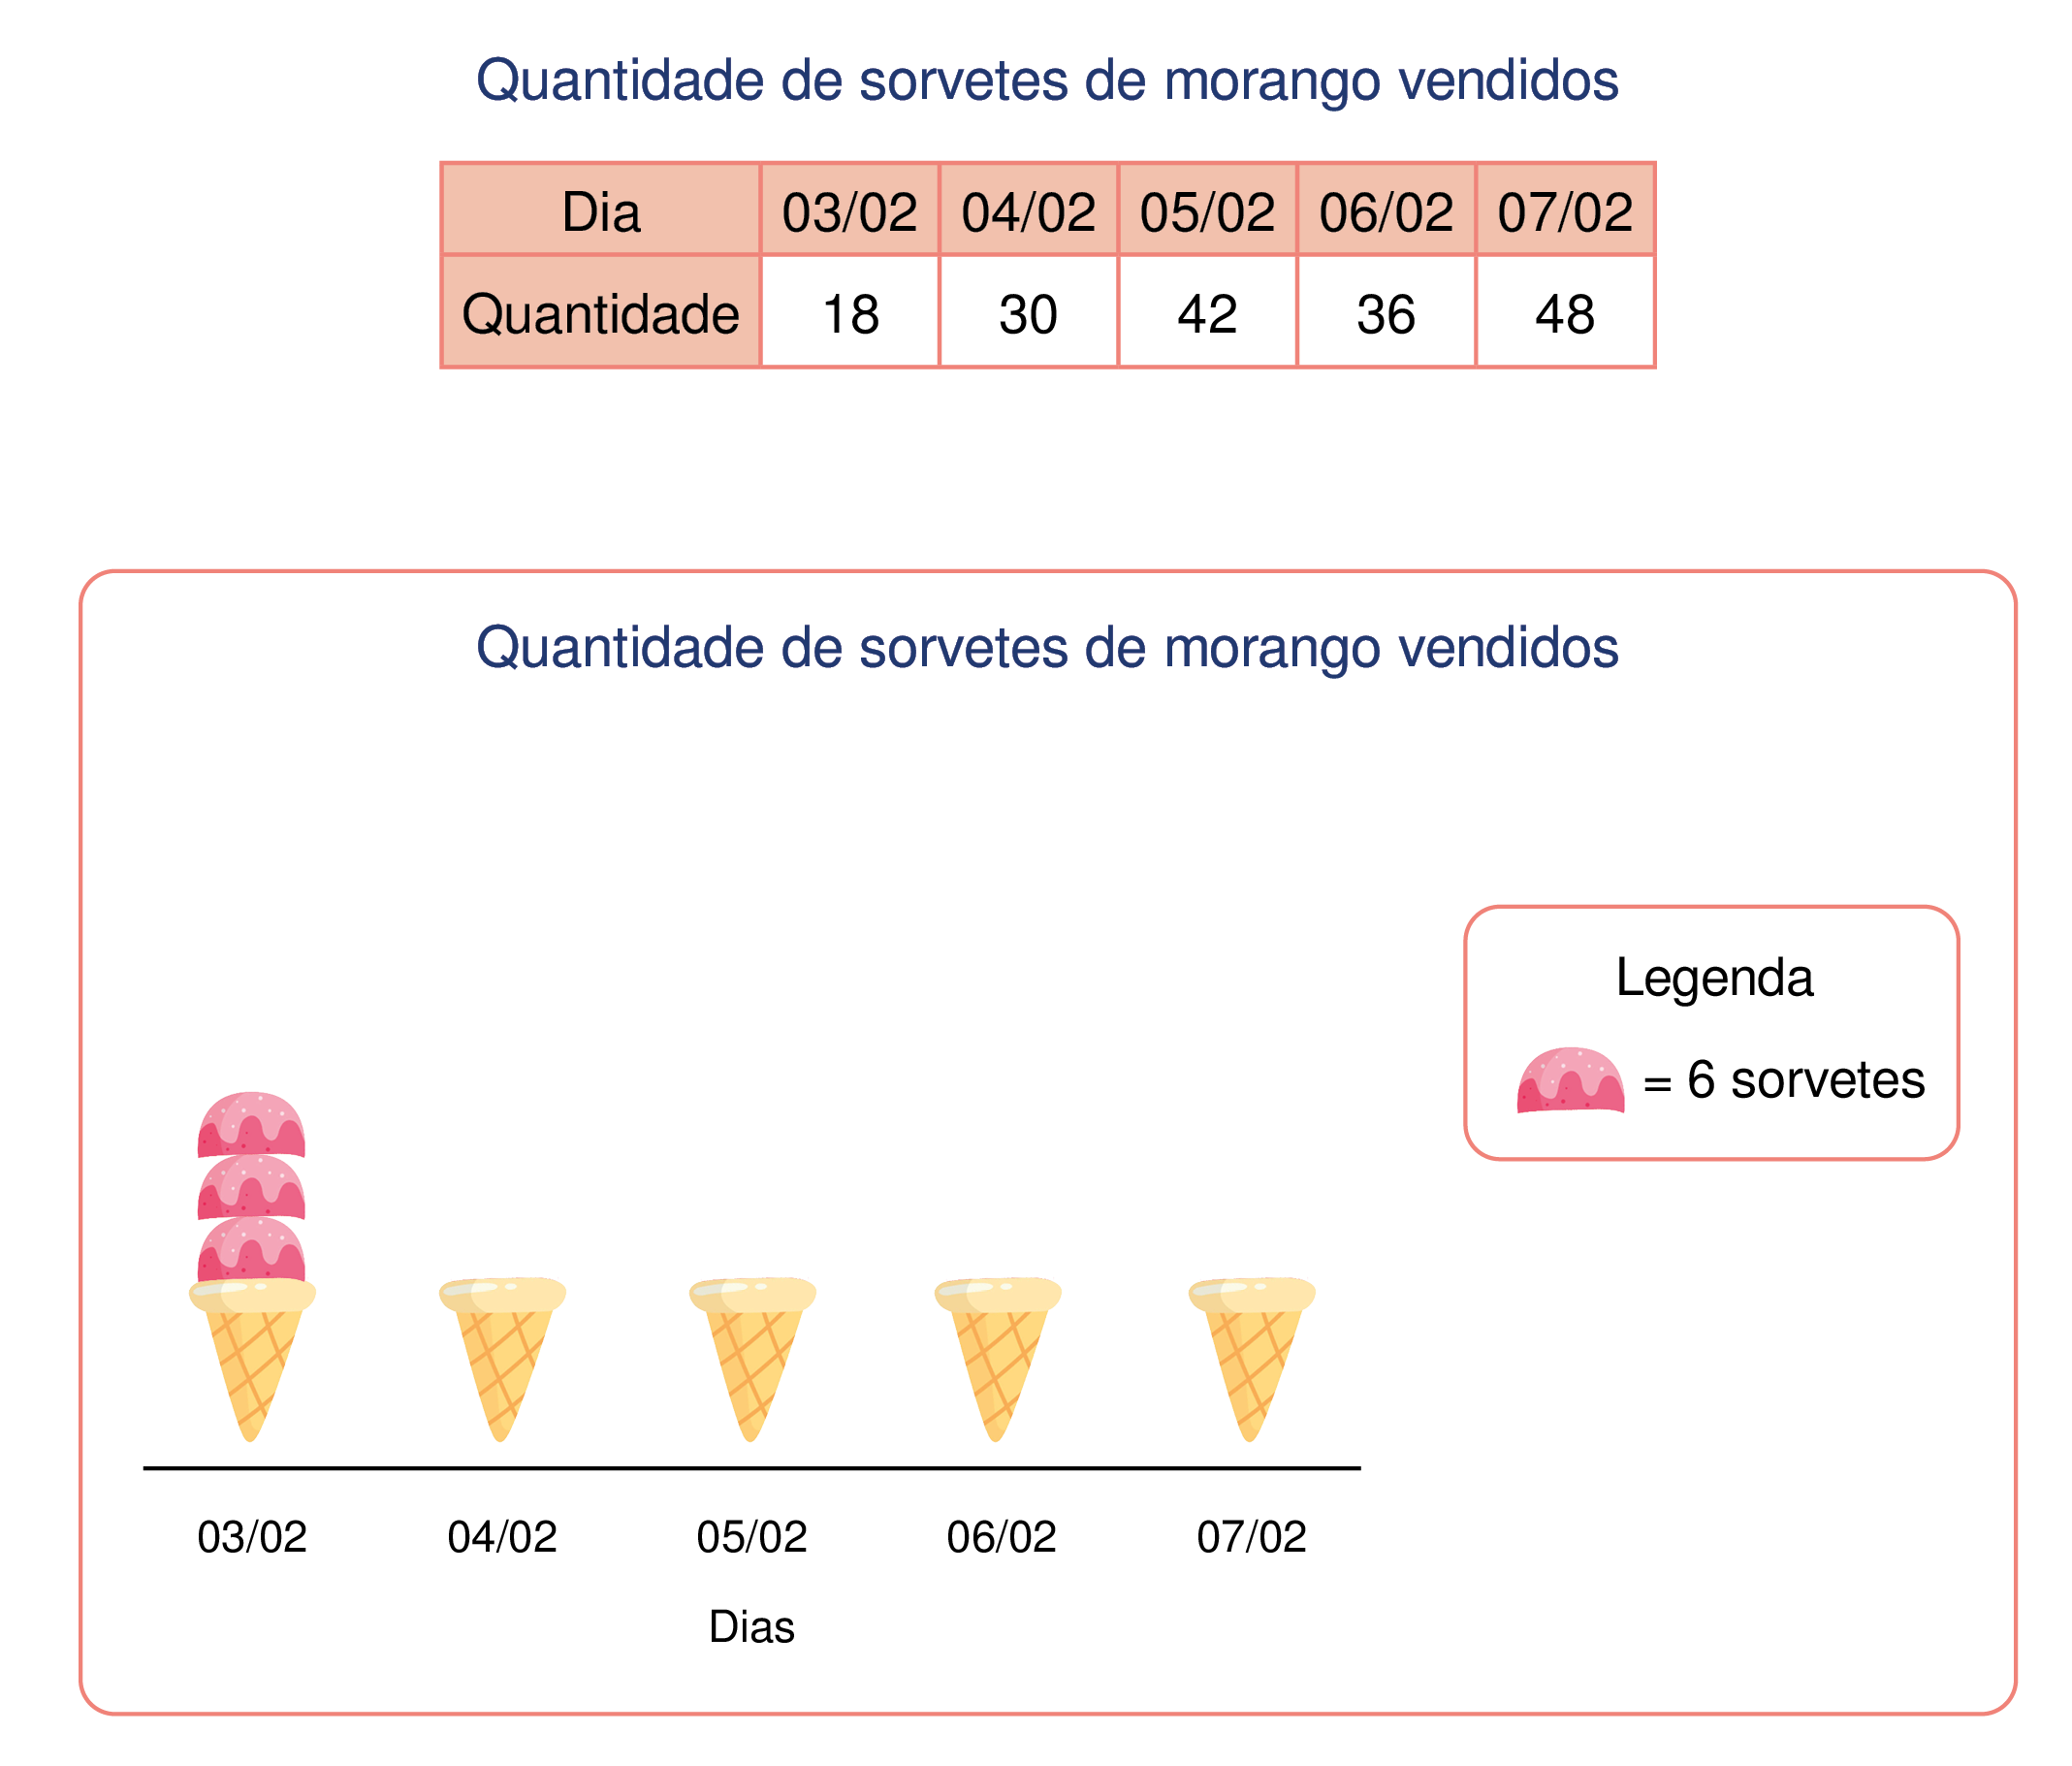
\includegraphics[width=\textwidth]{./media/image84.png}
\end{figure}

Utilizando os dados da tabela e a legenda que o gráfico fornece,
complete o gráfico, desenhando as bolas de sorvete que faltam.
\reduline{No sorvete do dia 04/02 deveremos ter 5 bolas de sorvete, já que cada
bola representa 6 sorvetes. No sorvete do dia 05/02 deveremos ter 7 bolas de sorvete, já que cada
bola representa 6 sorvetes. No sorvete do dia 06/02 deveremos ter 6 bolas de sorvete, já que cada
bola representa 6 sorvetes. No sorvete do dia 07/02 deveremos ter 8 bolas de sorvete, já que cada
bola representa 6 sorvetes.\hfill}

\pagebreak

\num{10} Utilizando conceitos modernos de educação, a professora de Leonardo
pediu que seus alunos realizassem uma pesquisa com 50 pessoas acerca da
preferência delas sobre determinados esportes. Sabendo que cada pessoa
escolheu uma única opção, os dados da pesquisa foram colocados em uma tabela.

\begin{figure}[htpb!]
\centering
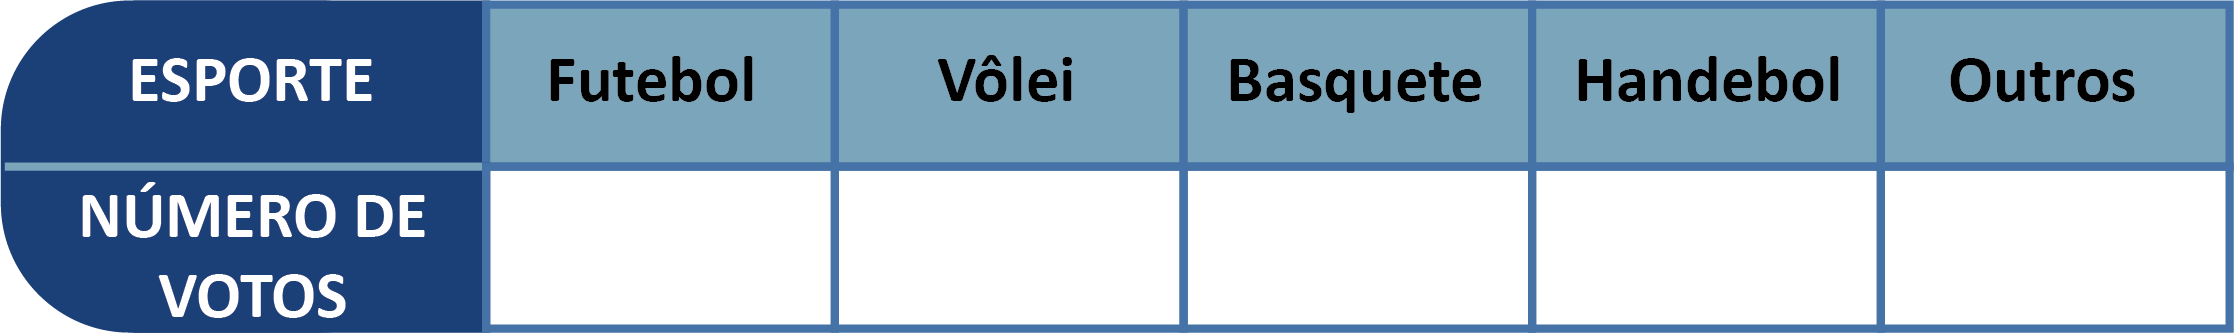
\includegraphics[width=\textwidth]{./media/image85.png}
\end{figure}

Em seguida, a professora pediu que os alunos contruíssem um gráfico de
colunas para representar os números da tabela. Construa o gráfico pedido
e ajude Leonardo a fazer a tarefa.

\begin{mdframed}[linewidth=2pt,linecolor=salmao]
\vspace{12cm}
\end{mdframed}

\pagebreak
\section*{Treino}

\num{1} Pelas regras de um processo seletivo, será aprovado 
o candidato que tirar todas as notas acima de 30 e, além disso, obtiver o maior
número de notas iguais. As notas de 4 candidatos foram colocadas na
tabela.

\begin{longtable}[]{@{}lllll@{}}
\toprule
\hline
\textbf{Candidato} & \textbf{Português} & \textbf{Matemática} & \textbf{Direito} &
\textbf{Informática}\tabularnewline
\midrule
\endhead
\textbf{A} & 33 & 33 & 33 & 34\tabularnewline
\hline
\textbf{B} & 32 & 39 & 32 & 40\tabularnewline
\hline
\textbf{C} & 24 & 37 & 40 & 42\tabularnewline
\hline
\textbf{D} & 36 & 16 & 26 & 40\tabularnewline
\hline
\bottomrule
\end{longtable}

Segundo as regras do concurso, qual será o candidato aprovado?

\begin{escolha}
\item
  A.
\item
  B.
\item
  C.
\item
  D.
\end{escolha}


\num{2} As notas de Geografia de 20 alunos foram organizadas em um quadro.

\begin{longtable}[]{@{}llllllllll@{}}
\toprule
7,0 & 5,0 & 9,0 & 5,0 & 8,0 & 5,0 & 8,0 & 9,0 & 10,0 &
8,0\tabularnewline
\midrule
\endhead
6,0 & 6,0 & 7,0 & 7,0 & 7,0 & 5,0 & 5,0 & 5,0 & 6,0 & 6,0\tabularnewline
\bottomrule
\end{longtable}

Quantos alunos obtiveram nota maior ou igual a 7,0?

\begin{multicols}{2}
\begin{escolha}
\item
  4.
\item
  10.
\item
  6.
\item
  16.
\end{escolha}
\end{multicols}

\pagebreak
\num{3} Uma escola fez uma pesquisa sobre os esportes preferidos de seus alunos
e os dados foram colocados em um gráfico.

\begin{figure}[htpb!]
\centering
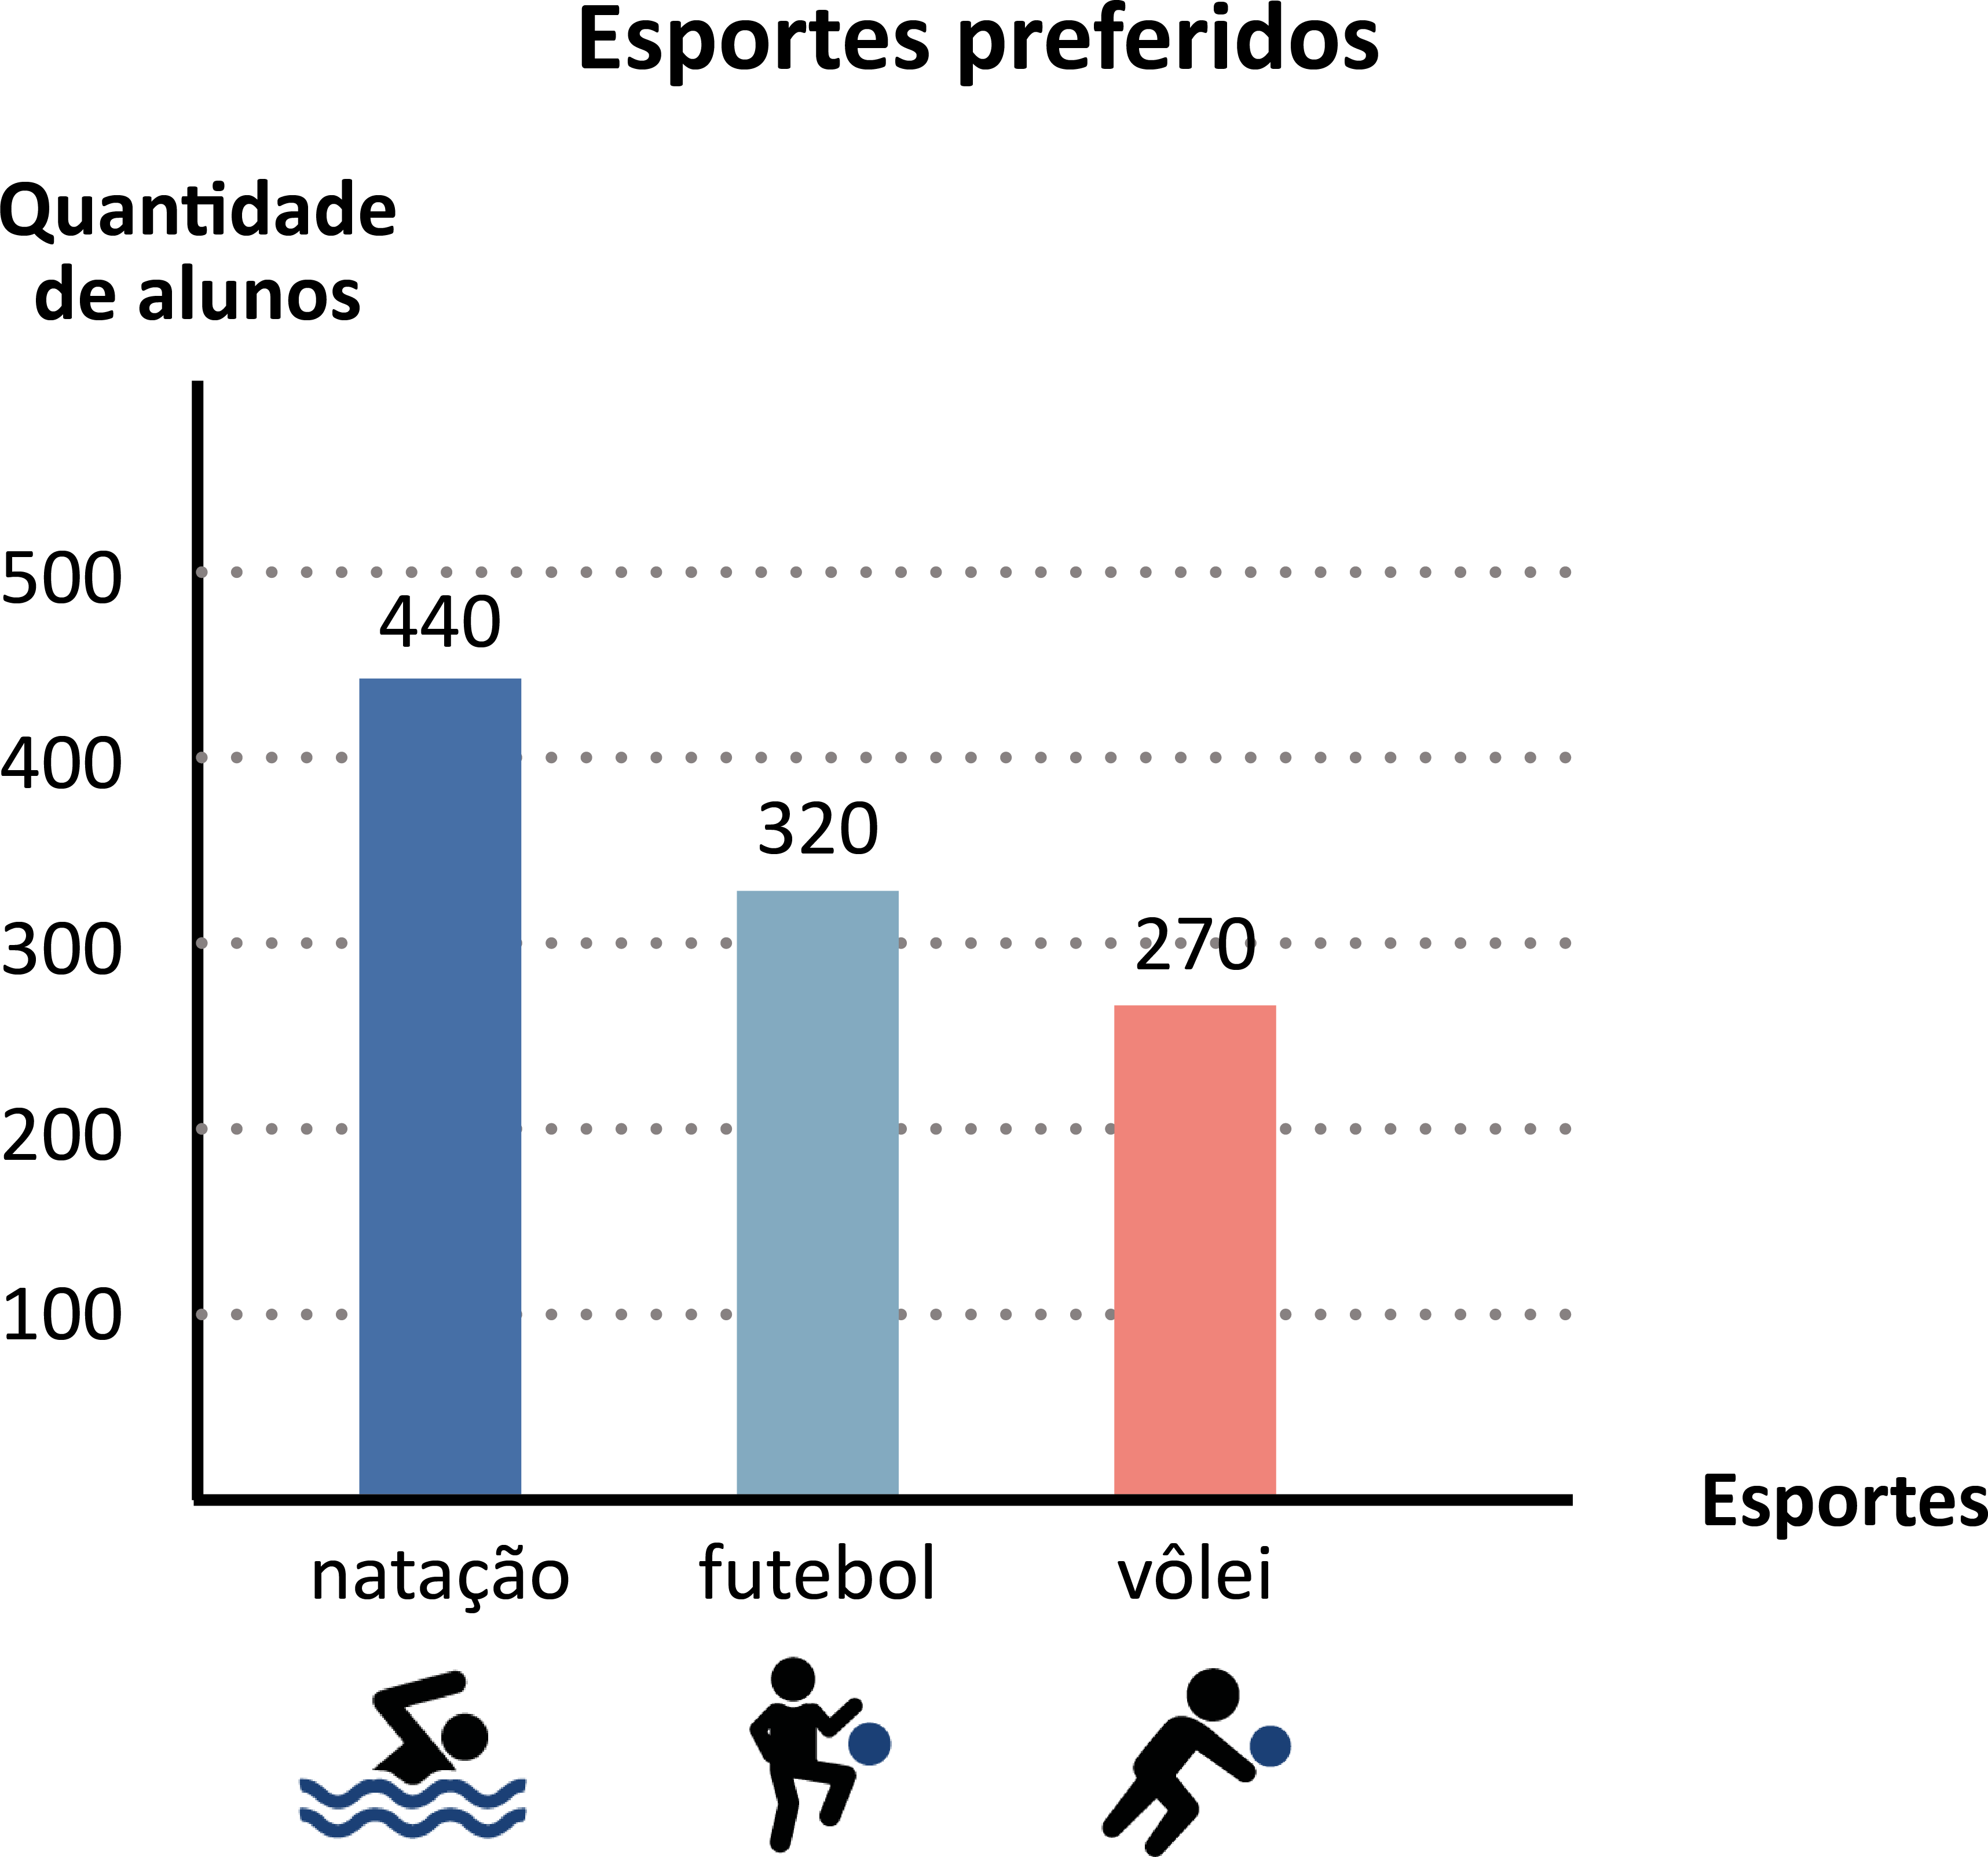
\includegraphics[width=\textwidth]{./media/image90.png}
\end{figure}

Sabendo-se que cada aluno escolheu uma única opção, pode-se dizer que o
número total de alunos que respondeu a essa pesquisa foi de

\begin{multicols}{2}
\begin{escolha}
\item
  1030.
\item
  760.
\item
  710.
\item
  590.
\end{escolha}
\end{multicols}

